\chapter{The Optimal Control Problem}
In previous chapter I have described how to build differential equations that
govern movement of a vehicle. This chapter describes two approaches of driving that vehicle optimally, first by using classical initial value problem/time marching formulation, then reformulating it to boundary value problem.

\section{Minimum maneuvering time problem as initial value problem }
The most common method for solving an ODE is as initial value problem.
An industry standard high fidelity multi-body time marching solver for vehicles is Car Maker from IPG \cite{ipg_carmaker}.
It is great for driving simulation, testing and development of advanced driver assistant systems, modeling the vehicles and racetrack modeling, it can be used for lap-time simulation, but with caveats.
In time marching solvers a separate controller is required, which becomes part of the ODE. This approach gives a solution to the problem of how to control car, so that it completes a lap around a circuit. However, this solution is almost certainly not optimal to time or any meaningful objective. Another issue is that if the vehicle's parameters change and the controller does not, the resulting time can be exactly same, because controller cannot take advantage of different vehicle's properties. Sensitivity analysis and lap time can be obtained but it is skewed by the chosen controller. The controller can be tuned for specific vehicle, but that will still not guarantee optimal control. Using time marching is not the best for sensitivity analysis and lap time simulation of a complex model. 

When the vehicles model is simplified to Quasi Steady State model, time marching simulation can be used.


%Another approach of solving controlled ODE is as 
%methods. Now the algorithm doesn't compute the states at only next time point,
%but it computes all states at all time points at the same time. Using this
%method it is possible to get rid of the controller, and instead of control rule
%a feed forward control vector along the trajectory is computed. This chapter
%deals with transcribing the continuos problem into discrete steps

\subsection{Quasi Steady state lap time simulation}
\label{QSS}
Following section describes commonly used algorithm which uses only initial value solvers, to compute the minimum maneuvering time.
For quasi steady state model \ref{QSS_model} it is possible to compute optimal speed profile ked dal som rovanke rovnice do nlp a dostal som rovnaky vysledok ako z toho algoritmu, takze aspon pre tuto trat to asi bude optimum speed profile using an algorithm well known among racing engineers. Figure \ref{fig:mass_point_speed_profile} shows thee speed profile obtained from this algorithm, on track from Figure \ref{fig:mass_point_speed_profile}, start is dot and cross is finish.
\begin{figure}[H]
    \centering
    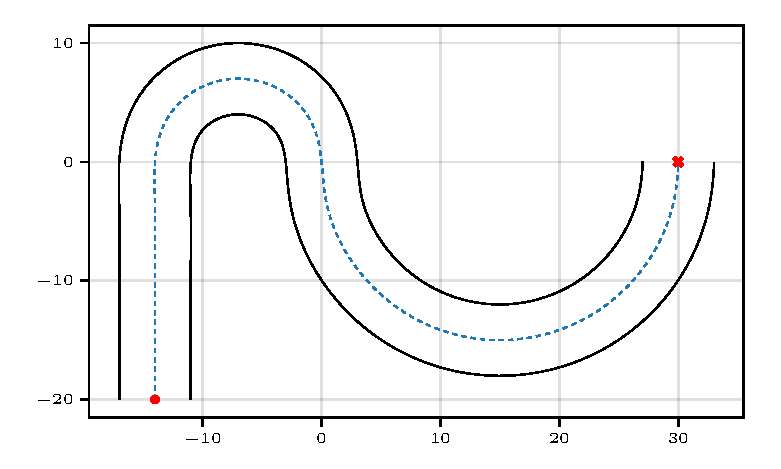
\includegraphics[width=1\textwidth]{../sync/massPointSteadyState/track.pdf}
    \caption{Test track used for the forward/backward pass example.}
    \label{fig:mass_point_track}
\end{figure}
\begin{figure}[H]
    \centering
    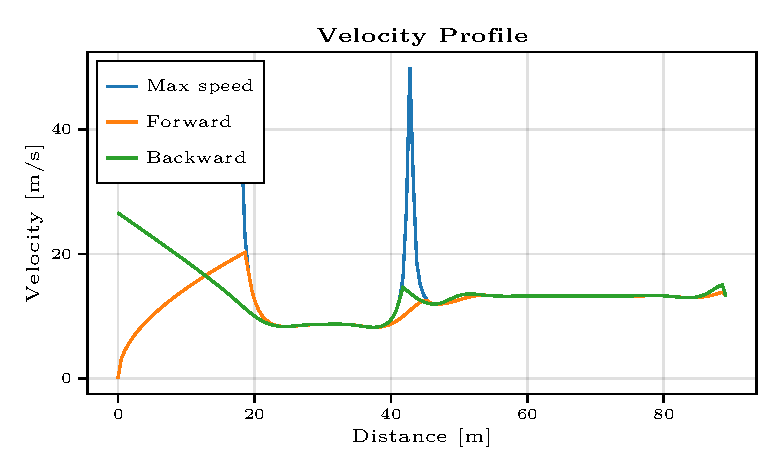
\includegraphics[width=1\textwidth]{../sync/massPointSteadyState/speed_profile.pdf}
    \caption{Speed profile from forward and backward passes with Quasi Steady state model}
    \label{fig:mass_point_speed_profile}
\end{figure}
Algorithm works in following manner:
\begin{enumerate}
    \item Maximum speed Pass: From the vehicle model and curvature along track, compute the maximum speed, blue line on Figure \ref{fig:mass_point_speed_profile}
    \item Forward pass: consider only forward acceleration limits of the vehicle (braking force is unlimited), run the vehicle from start to finish along the trajectory, applying maximum longitudinal acceleration and respecting max speed limit, orange line on Figure \ref{fig:mass_point_speed_profile}
    \item Consider only braking acceleration limits of the vehicle (acceleration force is unlimited), run the vehicle \emph{backwards, from finish to start} along the trajectory, applying maximum braking acceleration (braking now increases speed as the simulation is flipped)and respecting max speed limit
    \item Take minimum speeds of forward and backward pass and this gives the minimum time speed profile
\end{enumerate}
More complete description of this algorithm is in \cite{casanovaMinimumTimeVehicle2000}
This is the classic approach to minimum maneuvering time problem, the issue is that the trajectory of vehicle on track is fixed and cannot be optimized, the vehicle model must be heavily simplified, it does not work with any integral constraints like accumulator energy. However, the computation time can be fraction of a second for the entire lap. Tools using this method have proven to be extremely useful and many different analyses can be performed by leveraging its computational speed,for example varying the friction coefficient at on each corner, a corners importance on lap time can be calculated \cite{optimumg_corner_importance}. 
\section{Transcription methods}
Previous section described automotive specific methods of solving minimum maneuvering time problem, this section explains methods of transcribing the problem into the language of optimal control problem.
Transcription methods rewrite continuous (infinite-dimensional) OCP into finite-dimensional NLP.\@ That means representing the continuous trajectory of a state by values sampled at discrete points.
The terminology of transcription methods can be difficult to understand, as it is complex topic and often articles present conflicting information~\cite{kelly_traj_opt_terminology}. Website~\cite{kelly_traj_opt_terminology} and other work from Matthew Kelly~\cite{kelly_traj_opt_video,kelly_homepage,doi:10.1137/16M1062569} offers a very digestible introduction into the topic. This thesis focuses only on direct methods. Classification of methods in this thesis is based on~\cite{kelly_traj_opt_terminology} Figure~\ref{fig:ocp_methods_taxonomy} shows how transcription methods are commonly classified.

\begin{figure}[H]
\centering
\resizebox{\textwidth}{!}{%
\begin{tikzpicture}[
  >={Latex[length=2mm]},
  every node/.style={align=center},
  root/.style={draw, font=\footnotesize, text width=3.0cm, minimum height=0.8cm, inner sep=3pt},
  top/.style={draw, font=\footnotesize, text width=2.8cm, minimum height=1.0cm, inner sep=3pt},
  mid/.style={draw, font=\scriptsize, text width=2.6cm, minimum height=1.1cm, inner sep=3pt},
  leaf/.style={draw, font=\scriptsize, text width=2.0cm, minimum height=0.9cm, inner sep=2pt}
]
% --- Root ---
\node[root] (ocp) at (4.25, 0) {Continuous Time Optimal Control};

% --- Top-level branches: Direct on the left, Indirect center, HJB on the right ---
\node[top] (direct)   at (-1.0, -2.0) {Direct Methods:\\\textit{Transform into Nonlinear Program (NLP)}};
\node[top] (indirect) at ( 2.5, -2.0) {Indirect Methods, Pontryagin:\\\textit{Solve Boundary Value Problem}};
\node[top] (hjb)      at ( 6.0, -2.0) {Hamilton--Jacobi--Bellman Equation:\\\textit{Tabulation in State Space}};

\draw[->] (ocp.south) -- (direct.north);
\draw[->] (ocp.south) -- (indirect.north);
\draw[->] (ocp.south) -- (hjb.north);

% --- Direct children: shooting methods adjacent on the left, collocation on the right ---
\node[mid] (dss)  at (-4.0, -4.5) {Direct Single Shooting:\\\textit{Only discretized controls in NLP}\textit{}};
\node[mid] (dms)  at (-1.0, -4.5) {Direct Multiple Shooting:\\\textit{Controls and node start values in NLP}\textit{}};
\node[mid] (dcol) at ( 2.5, -4.5) {Direct Collocation:\\\textit{Discretized controls and states in NLP}\textit{}};

\draw[->] (direct.south) -- (dss.north);
\draw[->] (direct.south) -- (dms.north);
\draw[->] (direct.south) -- (dcol.north);

% --- Bottom leaves ---
\node[leaf] (erk1) at (-4.0, -6.7) {Explicit RK\\\textit{(integrator)}};
\node[leaf] (erk2) at (-1.0, -6.7) {Explicit RK\\\textit{(integrator)}};
\node[leaf] (hm)   at ( 1.4, -6.7) {$h$-methods\\\textit{low order,}\\\textit{many segments}};
\node[leaf] (pm)   at ( 3.6, -6.7) {$p$-methods\\\textit{high order,}\\\textit{few segments}};

\draw[->] (dss.south)  -- (erk1.north);
\draw[->] (dms.south)  -- (erk2.north);
\draw[->] (dcol.south) -- (hm.north);
\draw[->] (dcol.south) -- (pm.north);

\end{tikzpicture}%
}
\caption{Tree of approaches to continuous-time optimal control, adapted from~\cite{grosNumericalOptimalControla}, with the direct-methods branch expanded.}
\label{fig:ocp_methods_taxonomy}
\end{figure}

\subsection{Shooting methods}
Shooting methods get their name from aiming artillery canon analogy, with given powder load canon and target location find the aiming angle to hit the target. In depth explanation with animation and example code is here~\cite{kelly_cannon} This is classical boundary value problem. Methods shoot, miss, adjust aim, shoot again and iterate until target is hit. These methods are solving boundary value problem using an IVP solver. More precisely,
\begin{enumerate}
  \item Guess the controls
  \item Compute the solution using an initial value problem solver
  \item Compare the simulated value at the end of interval from 2.~with the boundary value(targets location)
  \item Based on error update the controls and go to 2.
\end{enumerate}

Shooting methods are split into single and multiple shooting. They differ in way they handle state discretisation. Single shooting discretizes the state only at start and end of interval and computes the trajectory in one shot. Whereas multiple shooting discretizes the states along the trajectory and computes multiple shots, this can be also parallelized on a CPU~\cite{FANG2022110926}. Shooting methods are progressively being displaced by collocation methods~\cite{raoSurveyNumericalMethods2010}

\subsection{Nonlinear Programming with Runge Kutta constraints}
These methods are not using initial value solvers to solve boundary value problem, instead they use nonlinear programming.
Most straightforward method to transcribe continuos optimal control problem
into non-linear program, is to use explicit Runge Kutta solving methods from
initial value problem as equality constraints on the dynamics of a vehicle. Using
Euler method, the constraints for the dynamics of vehicle are:
\begin{equation}
    \mathbf{x}_{k+1} = \mathbf{x}_k + h \cdot f(\mathbf{x}_k, \mathbf{u}_k),
\end{equation}
where $f$ denotes the vehicle dynamics, $h$ the step size, and $\mathbf{x}$ the state vector.
This works, but it may be the worst possible transcription method, due to high error and instability of euler method \cite{SolvingOrdinaryDifferential1987}. Problems of euler method encountered when solving initial value problems also translate to nonlinear programming. Implict RK methods can be used too, In Initial value problems they are used less often, as they require iterative solving. Optimal control problem is Boundary value problem and not initial value problem, therefore:

\begin{quote}
    \ldots for a boundary value problem \ldots any scheme becomes effectively implicit. Thus, the distinction between explicit and implicit initial value schemes becomes less important in the BVP context.
\end{quote}
\cite[p.~69]{Ascher1995}

For boundary value problem it makes no sense to use explicit Runge Kutta
methods, as they have inferior stability compared to implicit Runge Kutta
methods.\cite[p.~4]{raoSurveyNumericalMethods2010}. Implicit Runge Kutta methods, which are commonly used are from LobattoIIIA family, but any other method can be used. Book \cite{betts} uses
only these.

\subsection{Collocation methods}
\begin{quote}
    The concept of collocation is old and universal in numerical analysis \ldots For ordinary differential equations it consists in searching for a polynomial of de-gree s whose derivative coincides ("co-locates") at s given points with the vectorfield of the differential equation \ldots
    \cite[p.~224]{hairer}
\end{quote}
The article \cite{kelly_traj_opt_video} is an introductory explanation of inner working and implementation  of direct collocation methods, theory here is based on it and on \cite{garg_overview_nodate}. More in depth theory behind these methods was developed by Lloyd N. Trefethen in \cite{trefethenApproximationTheoryApproximation} and implementation in \cite{SpectralMethodsinMatlab}.
Collocation methods are a subset of implicit Runge-Kutta methods. The distinguishing property is that the solution of a boundary value problem is approximated by a piecewise polynomial in the independent variable (distance along the centerline). On each interval the polynomial is fixed by requiring it to satisfy the ODE exactly at $N$ chosen points the collocation nodes. 


There are numerous ways to construct a collocation method, in optimal control the classic methods are those based on roots Legendre or Chebyshev type I polynomials, Lagrange  polynomials \cite{ELGINDY199535, gargUnifiedFrameworkNumerical2010} and Gauss quadrature rule. In this thesis only Legendre and Gauss quadrature based collocation methods are covered. Figure \ref{fig:transcription_layer} depicts multiple ways of constructing collocation methods.

\begin{figure}[H]
\centering
\begin{tikzpicture}[
  >={Latex[length=2mm]},
  node distance=0.55cm and 0.18cm,
  basis/.style={draw, text width=1.4cm, minimum height=0.8cm, align=center, font=\scriptsize, inner sep=2pt},
  scheme/.style={draw, text width=3.2cm, minimum height=0.8cm, align=center, font=\small, inner sep=3pt},
  form/.style={draw, text width=1.25cm, minimum height=0.6cm, align=center, font=\scriptsize, inner sep=2pt},
  layer/.style={draw, minimum height=0.8cm, inner sep=4pt, align=center, font=\normalsize\bfseries}
]

\node[basis]                    (cheb) {Chebyshev\\I \& II};
\node[basis, right=of cheb]     (her)  {Hermite};
\node[basis, right=of her]      (lag)  {Laguerre};
\node[basis, right=of lag]      (leg)  {Legendre};
\node[basis, right=of leg]      (alag) {Assoc.\\Laguerre};
\node[basis, right=of alag]     (geg)  {Gegenbauer};
\node[basis, right=of geg]      (jac)  {Jacobi};

\node[layer, above=1cm of $(cheb.north)!0.5!(jac.north)$] (trans)
  {Orthogonal polynomials};

\foreach \n in {cheb,her,leg,lag,alag,geg,jac}
  \draw[->] (trans.south) -- (\n.north);

\node[scheme, below=1.8cm of leg] (lgr) {Legendre--Gauss--Radau\\(LGR) Quadrature};
\node[scheme, left=of lgr]   (lg)  {Legendre--Gauss\\(LG) Quadrature};
\node[scheme, right=of lgr]  (lgl) {Legendre--Gauss--Lobatto\\(LGL) Quadrature};

\draw[->] (leg.south) -- (lg.north);
\draw[->] (leg.south) -- (lgr.north);
\draw[->] (leg.south) -- (lgl.north);

\foreach \n in {cheb,her,lag,alag,geg,jac}
  \node[font=\Large, below=0.35cm of \n] {$\vdots$};

\foreach \parent in {lg,lgr,lgl}{
  \node[form, below=0.8cm of \parent, xshift=-0.85cm] (\parent-int)  {Integral};
  \node[form, below=0.8cm of \parent, xshift=0.85cm]  (\parent-diff) {Differ.};
  \draw[->] (\parent.south) -- (\parent-int.north);
  \draw[->] (\parent.south) -- (\parent-diff.north);
}

\end{tikzpicture}
\caption{Collocation transcription methods}
\label{fig:transcription_layer}
\end{figure}

\subsubsection{Lagrange polynomial}
First part of creating a collocation method is creating an interpolating polynomial basis,
\begin{equation}
    L_i(\tau) = \prod_{\substack{j=0 \\ j \neq i}}^{N} \frac{\tau - \tau_j}{\tau_i - \tau_j}, \qquad i = 0, \ldots, N.
    \label{legendre}
\end{equation}
Where $\tau$ is the point to be interpolated and $\tau_j$ and $\tau_i$ are node positions, in order to get interpolating polynomial $L(\tau)$, values at nodes $x_j$ are multiplied by corresponding Lagrange base and summed
\begin{equation}
    L(\tau) = \sum_{i=0}^{N} f_{i} L_i(\tau).
\end{equation}
Now it is possible to interpolate a state between the discretized nodes, Note that the node locations for Legendre polynomial are arbitrary. In the actual implementation, calculation of polynomial basis from definition \ref{legendre} is numerically impractical, therefore barycentric form from \cite{berrutBarycentricLagrangeInterpolation2004} has been used as implementation of these methods. The next step is to compute definite integral using values from function values at nodes.
%This creates a unique polynomial of lowest degree that interpolates a given set of data. The data points or nodes can be chosen arbitrary.
%A general RK method only yields state values at the stage points.
%Node choice is not arbitrary, nodes have to be selected in a special manner in order for second property of collocation to work. that is quadrature rule.
\subsubsection{Gaussian Quadrature rule}
Quadrature rule is the approximation of definite integral of a function by a sum of function values at given nodes. In optimal control context Gaussian quadrature is commonly used
\begin{equation}
    \int_{-1}^{1} f(\tau)\,\mathrm{d}\tau \approx \sum_{i=0}^{n} w_i \, f_i,
    \label{eq:gauss_quadrature}
\end{equation}
where $w$ are Gaussian quadrature weights.
A useful property of Gaussian quadrature of order $N$ is that it approximates the integral to machine precision whenever the integrated function is a polynomial of degree at most $2N-1$. Node selection for Gauss quadrature is \emph{not arbitrary}, in collocation methods the node positions are based on roots of Legendre polynomial. Node positions specify the type of collocation method and are creating in following manner.
%Pairing Gauss quadrature with Legendre polynomials creates a collocation method. Commonly used collocation methods constructed using Legendre polynomials and Gauss quadrature are constructed in following manner.
Let $P_N(\tau)$ denote the Legendre polynomial of degree $N$. Three node families are commonly used~\cite{garg_overview_nodate}:
\begin{itemize}
    \item Legendre-Gauss: roots of $P_N(\tau)$, includes no endpoints.
    \item Legendre-Gauss-Radau: roots of $P_{N-1}(\tau) + P_N(\tau)$, includes one endpoint.
    \item Legendre-Gauss-Lobatto: roots of $\dot{P}_{N-1}(\tau)$, includes both endpoints.
\end{itemize}

\begin{figure}
    \centering
    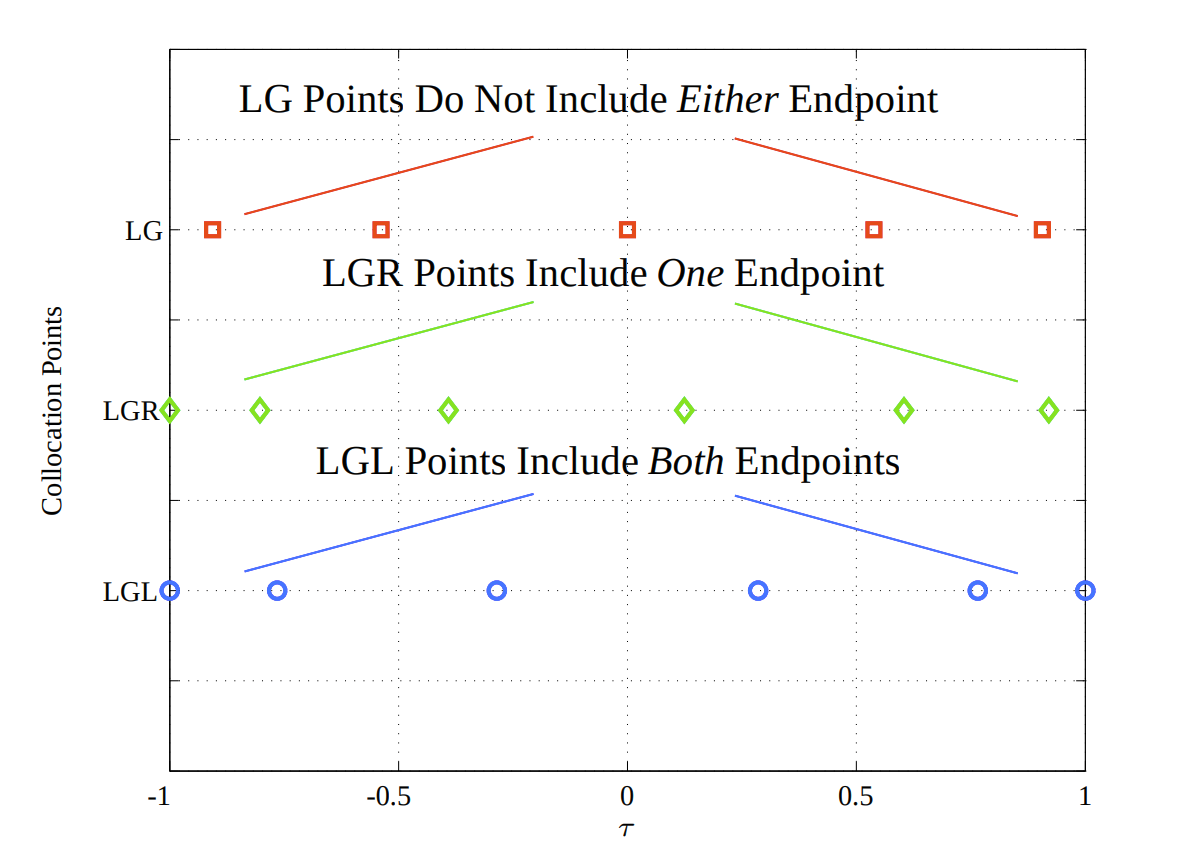
\includegraphics[width=0.75\linewidth]{../sync/image.png}
    \caption{Schematic Showing the Differences Between LGL, LGR, and LG Collocation Points, taken from \cite{garg_overview_nodate}}
    \label{fig:placeholder}
\end{figure}

\section{Collocation at Legendre-Gauss points}
%Legendre polynomials are paired with Gauss quadrature to create a collocation method.
%where $w_i$ are the quadrature weights and $f_i = f(\tau_i)$ are samples at the nodes. Because collocation and quadrature share nodes, quadrature of the collocation polynomial is exact up to the appropriate polynomial degree.
%https://en.wikipedia.org/wiki/Classical_orthogonal_polynomials#Table_of_classical_orthogonal_polynomials
%Collocation methods are the core of this thesis, I have implemented  Gauss radau, gauss, gauss lobatto. Collocation methods differ in points at which the derivative of polynomial coincides ("co-locates) with the vector field of differential equation. Commonly used methods in optimal control are radau, lobatto, legendre. They can be written in integral and differential form\cite{garg_overview_nodate}. Collocatiom methods in this thesis are based on Framework described in\cite{gargUnifiedFrameworkNumerical2010}

%Polynomial that aproximates the solution of ODE is based on Legendre polynomials.
Legendre-Gauss collocation methods uses nodes strictly inside the interval for approximation using polynomial.
With $N$ nodes, it is possible to approximate functions up to degree $N-1$ with machine precision.
States are approximated by series
\begin{equation}
    x^N_j(\tau) = \sum_{i=0}^{N} x_{ij}\, L_i(\tau),
\end{equation}
where $j$ is the number of the state.
Then the series is differentiated using barycentric form from~\cite[p.513]{berrutBarycentricLagrangeInterpolation2004} and evaluated at $k$-th collocation point $\tau_k$
\begin{equation}
    \dot{x}^N_j(\tau_k) = \sum_{i=0}^{N} x_{ij}\, \dot{L}_i(\tau_k) = \sum_{i=0}^{N} D_{ki}\, x_{ij}, \qquad D_{ki} = \dot{L}_i(\tau_k).
\end{equation}
Matrix $\mathbf{D} $is called \emph{Gauss Pseudospectral differentiation matrix}. In matrix notation can be written
\begin{equation}
\mathbf{DX} = \mathbf{F(X_{\mathrm{LG}}, U_{\mathrm{LG}})    }
\end{equation}
where $\mathbf{X_{LG}}$ is matrix of states at Legendre-Gauss node points, $\mathbf{U_{LG}}$ is matrix of controls at Legendre-Gauss node points, $\mathbf{X}$ is matrix of states at Legendre-Gauss node points and at initial point $x_0$

%then the output?? of differential equation can be aproximated using the
%differentiation matrix.
%\begin{equation}
%    \dot{x}^N_j(\tau_i) = (D\mathbf{X})_{ij}
%\end{equation}
This is then used as constraints to formulate a transcription method
\begin{equation}
    \begin{aligned}
        \min \quad        & \Phi(\mathbf{X}_{N+1})                         ,                                                \\
        \text{s.t.} \quad & \mathbf{DX} = \mathbf{F}(\mathbf{X}_\text{LG},\, \mathbf{U}_\text{LG})      ,                            \\
                          & \mathbf{X}_{N+1} = \mathbf{X}_0 + \mathbf{w^T} \mathbf{F}(\mathbf{X}_\text{LG},\, \mathbf{U}_\text{LG}), \\
                          & \mathbf{X}_0 = \mathbf{x}_0.
    \end{aligned}
\end{equation}
Where $w$ are the Gauss quadrate weights.
This is the differential form of Legendre-Gauss collocation method, integral from is described in \cite{gargUnifiedFrameworkNumerical2010}.
\section{Collocation at Legendre-Gauss-Radau points}
This method is constructed in similar manner to previous, with difference that one endpoint is a collocation node. This is an advantage, as the resulting nonlinear programming formulation does not require the gauss quadrature rule for endpoint and it is smaller.
This method approximates functions up degree $2N-2$ with machine precision, this is lower precision than Legendre-Gauss.
\begin{equation}
\begin{aligned}
\min \quad & \Phi(\mathbf{X}_N) \\
\text{subject to} \quad & \mathbf{D}\mathbf{X} = \mathbf{F}(\mathbf{X}^{\mathrm{LGR}}, \mathbf{U}^{\mathrm{LGR}}), \\
& \mathbf{X}_0 = \mathbf{x}_0.
\end{aligned}
\end{equation}
This is also a differential formulation.
\section{Collocation at Legendre-Gauss-Lobatto points}
The Gauss-Lobatto family includes both endpoints as collocation nodes and has a quadrature degree of exactness $2N-3$. It contains classical low-order schemes like the trapezoidal rule and Hermite--Simpson. I implement it using the Butcher tableau of LobattoIIIA implicit Runge--Kutta methods from \cite{ehlePadeApproximationsExponential}.

The dynamics is collocated at $N$ LobattoIIIA nodes $c_i \in [-1,1]$ with coefficient matrix $a_{ij}$ taken from the Butcher tableau. $\mathbf{X}_i$ and $\mathbf{U}_i$ are the state and control at node $i$, placed at $\tau_i = c_i h/2$, where $h$ is the length of the interval. The node constraints are
\begin{equation}
    \mathbf{X}_i = \mathbf{X}_0 + \frac{h}{2} \sum_{j=1}^{N} a_{ij}\, \mathbf{F}(\mathbf{X}_j, \mathbf{U}_j), \qquad i = 2, \dots, N,
\label{eq:lobattoIIIA-stage}
\end{equation}
where $\mathbf{X}_0$ is the left endpoint.
The resulting NLP is
\begin{equation}
\begin{aligned}
\min \quad & \Phi(\mathbf{X}_N) \\
\text{subject to} \quad & \mathbf{X}_i = \mathbf{X}_0 +  \sum_{j=1}^{N} a_{ij}\, \mathbf{F}(\mathbf{X}_j, \mathbf{U}_j), \quad i = 2, \dots, N, \\
& \mathbf{X}_0 = \mathbf{x}_0.
\end{aligned}
\end{equation}
This is an integral formulation of collocation method, in book \cite{betts} trapezoidal and Hermite-Simpson methods written in this form.

%\section{Gauss methods as pseudospectral collocation}
%I have implemented Gauss-Legendre, Gauss-Lobatto, Gauss-Radau as global collocation methods, that is one polynomial approximating the entire trajectory. I have implemented them according to~\cite{garg_overview_nodate}
%\section{Gauss methods as h-method}
%\subsection{collocation integral form}
%integral form is straight forward, same as other unge kutta Methods
%\subsection{collocation differential form}
%differeanital form requires to create differentiation matrix of the
%aproximating polnomial,which contains the difference of the approximating
%polynomial.

\subsection{h and p methods for collocation}
A function can be approximated in three ways. The first uses a single high-order polynomial over the entire trajectory, these are p methods. The second uses many piecewise continuous polynomials of low and fixed order, as in \cite{betts}, these are h methods. The third combines both ideas, using many polynomials whose order is allowed to vary between segments, these are hp methods. The Legendre-Gauss, Legendre-Gauss-Radau and Legendre-Gauss-Lobatto schemes presented above are the building blocks for all three categories. A single global instance gives a p method. Chaining many low-order instances on consecutive intervals with continuity at the shared endpoints gives an h method. Chaining instances of different orders gives an hp method.

Intuitively p methods should suffer from the Runge phenomenon, but they do not. The discretization nodes are not equispaced, they are clustered toward the endpoints, which suppresses the oscillations. Methods based on roots of Chebyshev polynomials suppress the Runge phenomenon better than Legendre methods\cite{trefethenApproximationTheoryApproximation}.
\section{Mesh refinement methods}
Mesh refinement works by changing polynomial order and number and place of segements. In mesh refinemnt it is also important to remove segments that are unecessary. Mesh refinemnt methods are divided into three categories.
\begin{figure}[H]
\centering
\begin{tikzpicture}[
  >={Latex[length=2mm]},
  node distance=0.7cm and 0.35cm,
  method/.style={draw, text width=2.4cm, minimum height=0.9cm, align=center, font=\small, inner sep=3pt},
  layer/.style={draw, minimum height=0.8cm, inner sep=4pt, align=center, font=\normalsize\bfseries}
]

\node[method]              (p)   {$p$-refinement\\(raise polynomial degree)};
\node[method, right=of p]  (h)   {$h$-refinement\\(subdivide segments)};
\node[method, right=of h]  (hp)  {$hp$-refinement\\(combination of h and p)};

\node[layer, above=1cm of $(p.north)!0.5!(hp.north)$] (mesh)
  {Mesh refinement strategy};

\foreach \n in {p,h,hp}
  \draw[->] (mesh.south) -- (\n.north);

\end{tikzpicture}
\caption{Mesh refinement categories~\cite{darbyHpAdaptivePseudospectral2011,pattersonPhMeshRefinement2015}.}
\label{fig:mesh_refinement_layer}
\end{figure}



\subsection{P adaptive methods}
The p adaptive methods work by increasing the order of polynomial, until the error
is below user defined threshold. Figure \ref{fig:power_node_controls} shows that
error along track is not distributed equaly. Error is localised around areas
with large jump in controls. These areas need finer sampling. P methods cannot
focus these specific points directly, they focus entire trajectory.

The errors are concentrated around the discontinuity of controls, where the
behaviour of the vehicle is more complex/ requiring high order or finer
approximation see Figure \ref{fig:power_node_controls}. Time optimal control of car around track has many discontinuities and therefore p methods are not a good fit for this use.

\begin{figure}[H]
    \centering
    \makebox[\textwidth][c]{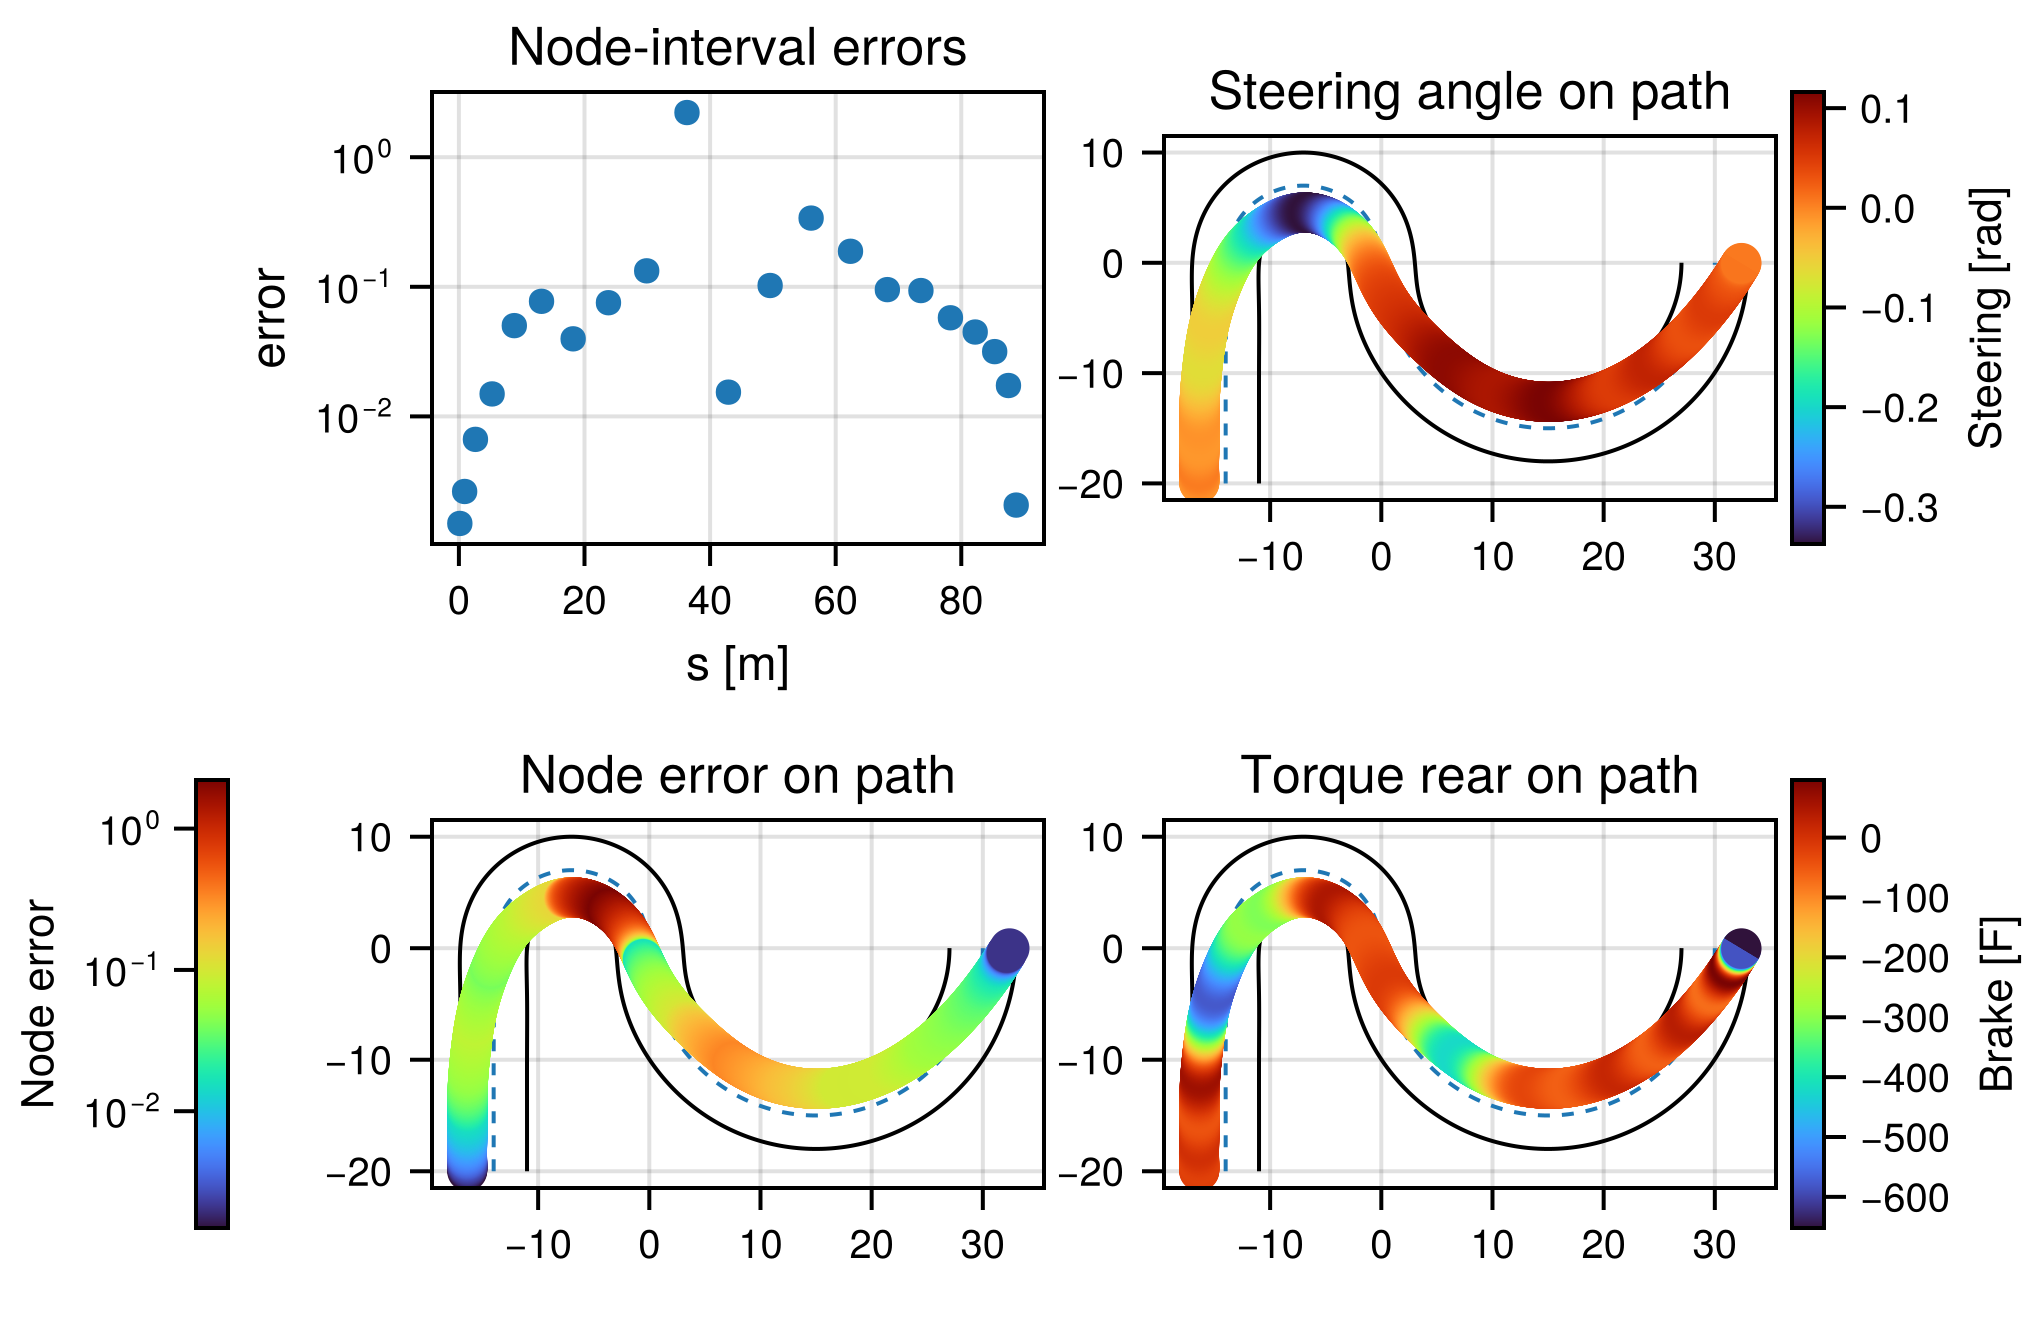
\includegraphics[width=1\textwidth]{../sync/p_methodplots/power_summary2x2.png}}
    \caption{Node-interval ODE error for power-test case.}
    \label{fig:power_node_controls}
\end{figure}

\subsection{h adaptive methods}
The h methods are used when solution of optimal control problem is approximated by
many intervals with low degree polynomial. These methods can decide to split
segment into two smaller segments, they use different techniques to do this.
Method described in \cite{betts} calculates error using Romberg quadrature with machine precision. Another
method described in \cite{jisongzhaoshuangliAdaptiveMeshRefinement} uses
techniques from essentially non oscillatory (ENO) interpolation

\begin{figure}[H]
    \centering
    \makebox[\textwidth][c]{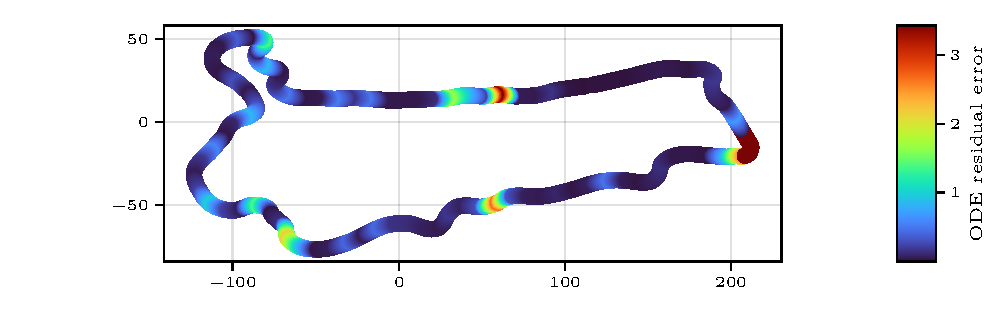
\includegraphics[width=1\textwidth]{../sync/thesisImages/mesh_refinement_fscz_error_iter0.pdf}}
    \caption{Node-interval ODE error for power-test case.}
    \label{fig:power_node_controls}
\end{figure}

\begin{figure}[H]
    \centering
    \makebox[\textwidth][c]{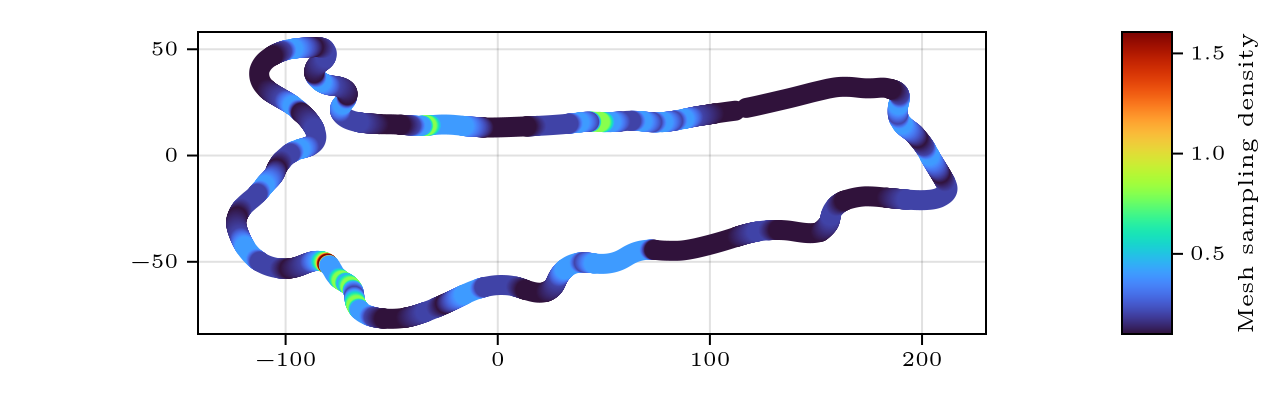
\includegraphics[width=1\textwidth]{../sync/thesisImages/mesh_refinement_fscz_density_iter10.png}}
    \caption{Node-interval ODE error for power-test case.}
    \label{fig:power_node_controls}
\end{figure}

\cite{Harten1997} to decide where to split and remove nodes.
\subsection{hp adaptive methods}
The hp adaptive methods are state of the art in mesh refinement. They are
combination of increasing/decreasing mesh segments and increasing/decreasing
order of approximating polynomial inside segments. One of the first hp-method
and commonly cited is decribed in
article~\cite{darbyHpAdaptivePseudospectral2011} from University of Florida.
They have produces numerous papers on hp- adaptive mesh
refinemnt~\cite{agamawiCGPOPSSoftwareSolving2020}
\cite{liuAdaptiveMeshRefinement2018}. Recent work on mesh refinemnt for
functions with kinks~\cite{wilkaAdaptiveHpPolynomialBased2025}. They are the
most complex for implementation and unfortunately I did not have the time to
implement them.

\section{Adjoint methods}
\label{sec:adjoint}

Adjoint methods allow for differentiating the solution of optimization problem.
In this case it is function of time on states and controls along the trajectory and car parameters This is very useful as it greatly simplifies sensitivity
analysis. Traditional way of sensitivity analysis is to compute several runs with
different vehicle parameters, but this allows to compute sensitivity of all
parameters in one shot. I am using DiffOpt.jl \cite{besancon2023diffopt}, it is
not exactly adjoint i dont really understand very well how it works.
